\documentclass[11pt,preprint, authoryear]{elsarticle}

\usepackage{lmodern}
%%%% My spacing
\usepackage{setspace}
\setstretch{1.2}
\DeclareMathSizes{12}{14}{10}{10}

% Wrap around which gives all figures included the [H] command, or places it "here". This can be tedious to code in Rmarkdown.
\usepackage{float}
\let\origfigure\figure
\let\endorigfigure\endfigure
\renewenvironment{figure}[1][2] {
    \expandafter\origfigure\expandafter[H]
} {
    \endorigfigure
}

\let\origtable\table
\let\endorigtable\endtable
\renewenvironment{table}[1][2] {
    \expandafter\origtable\expandafter[H]
} {
    \endorigtable
}


\usepackage{ifxetex,ifluatex}
\usepackage{fixltx2e} % provides \textsubscript
\ifnum 0\ifxetex 1\fi\ifluatex 1\fi=0 % if pdftex
  \usepackage[T1]{fontenc}
  \usepackage[utf8]{inputenc}
\else % if luatex or xelatex
  \ifxetex
    \usepackage{mathspec}
    \usepackage{xltxtra,xunicode}
  \else
    \usepackage{fontspec}
  \fi
  \defaultfontfeatures{Mapping=tex-text,Scale=MatchLowercase}
  \newcommand{\euro}{€}
\fi

\usepackage{amssymb, amsmath, amsthm, amsfonts}

\def\bibsection{\section*{References}} %%% Make "References" appear before bibliography


\usepackage[round]{natbib}

\usepackage{longtable}
\usepackage[margin=2.3cm,bottom=2cm,top=2.5cm, includefoot]{geometry}
\usepackage{fancyhdr}
\usepackage[bottom, hang, flushmargin]{footmisc}
\usepackage{graphicx}
\numberwithin{equation}{section}
\numberwithin{figure}{section}
\numberwithin{table}{section}
\setlength{\parindent}{0cm}
\setlength{\parskip}{1.3ex plus 0.5ex minus 0.3ex}
\usepackage{textcomp}
\renewcommand{\headrulewidth}{0pt}

\usepackage{array}
\newcolumntype{x}[1]{>{\centering\arraybackslash\hspace{0pt}}p{#1}}

%%%%  Remove the "preprint submitted to" part. Don't worry about this either, it just looks better without it:
\makeatletter
\def\ps@pprintTitle{%
  \let\@oddhead\@empty
  \let\@evenhead\@empty
  \let\@oddfoot\@empty
  \let\@evenfoot\@oddfoot
}
\makeatother

 \def\tightlist{} % This allows for subbullets!

\usepackage{hyperref}
\hypersetup{breaklinks=true,
            bookmarks=true,
            colorlinks=true,
            citecolor=blue,
            urlcolor=blue,
            linkcolor=blue,
            pdfborder={0 0 0}}


% The following packages allow huxtable to work:
\usepackage{siunitx}
\usepackage{multirow}
\usepackage{hhline}
\usepackage{calc}
\usepackage{tabularx}
\usepackage{booktabs}
\usepackage{caption}


\newenvironment{columns}[1][]{}{}

\newenvironment{column}[1]{\begin{minipage}{#1}\ignorespaces}{%
\end{minipage}
\ifhmode\unskip\fi
\aftergroup\useignorespacesandallpars}

\def\useignorespacesandallpars#1\ignorespaces\fi{%
#1\fi\ignorespacesandallpars}

\makeatletter
\def\ignorespacesandallpars{%
  \@ifnextchar\par
    {\expandafter\ignorespacesandallpars\@gobble}%
    {}%
}
\makeatother

\newlength{\cslhangindent}
\setlength{\cslhangindent}{1.5em}
\newenvironment{CSLReferences}%
  {\setlength{\parindent}{0pt}%
  \everypar{\setlength{\hangindent}{\cslhangindent}}\ignorespaces}%
  {\par}


\urlstyle{same}  % don't use monospace font for urls
\setlength{\parindent}{0pt}
\setlength{\parskip}{6pt plus 2pt minus 1pt}
\setlength{\emergencystretch}{3em}  % prevent overfull lines
\setcounter{secnumdepth}{5}

%%% Use protect on footnotes to avoid problems with footnotes in titles
\let\rmarkdownfootnote\footnote%
\def\footnote{\protect\rmarkdownfootnote}
\IfFileExists{upquote.sty}{\usepackage{upquote}}{}

%%% Include extra packages specified by user
\usepackage{booktabs}
\usepackage{longtable}
\usepackage{array}
\usepackage{multirow}
\usepackage{wrapfig}
\usepackage{float}
\usepackage{colortbl}
\usepackage{pdflscape}
\usepackage{tabu}
\usepackage{threeparttable}
\usepackage{threeparttablex}
\usepackage[normalem]{ulem}
\usepackage{makecell}
\usepackage{xcolor}

%%% Hard setting column skips for reports - this ensures greater consistency and control over the length settings in the document.
%% page layout
%% paragraphs
\setlength{\baselineskip}{12pt plus 0pt minus 0pt}
\setlength{\parskip}{12pt plus 0pt minus 0pt}
\setlength{\parindent}{0pt plus 0pt minus 0pt}
%% floats
\setlength{\floatsep}{12pt plus 0 pt minus 0pt}
\setlength{\textfloatsep}{20pt plus 0pt minus 0pt}
\setlength{\intextsep}{14pt plus 0pt minus 0pt}
\setlength{\dbltextfloatsep}{20pt plus 0pt minus 0pt}
\setlength{\dblfloatsep}{14pt plus 0pt minus 0pt}
%% maths
\setlength{\abovedisplayskip}{12pt plus 0pt minus 0pt}
\setlength{\belowdisplayskip}{12pt plus 0pt minus 0pt}
%% lists
\setlength{\topsep}{10pt plus 0pt minus 0pt}
\setlength{\partopsep}{3pt plus 0pt minus 0pt}
\setlength{\itemsep}{5pt plus 0pt minus 0pt}
\setlength{\labelsep}{8mm plus 0mm minus 0mm}
\setlength{\parsep}{\the\parskip}
\setlength{\listparindent}{\the\parindent}
%% verbatim
\setlength{\fboxsep}{5pt plus 0pt minus 0pt}



\begin{document}



\begin{frontmatter}  %

\title{Forecasting South African Financial Market Volatility with
Machine Learning}

% Set to FALSE if wanting to remove title (for submission)




\author[Add1]{Jonathan Rossouw}
\ead{20858345@sun.ac.za}







\begin{abstract}
\small{
Volatility modelling is an important problem in financial econmetrics.
The recent proliferation of powerful machine learning techniques offer
models that are well suited to this complex problem. In this paper
volatility forecasting of the JSE All Share index for different machine
learning techniques are compared. The Support Vector Regression (SVR)
and Long-Short Term Memory Recurrent Neural Networks (LSTM) are
compared. An EGARCH models is used as a baseline model. The LSTM model
performed best at one-day ahead and the SVR at three-day ahead
forecasting.
}
\end{abstract}

\vspace{1cm}





\vspace{0.5cm}

\end{frontmatter}



%________________________
% Header and Footers
%%%%%%%%%%%%%%%%%%%%%%%%%%%%%%%%%
\pagestyle{fancy}
\chead{}
\rhead{}
\lfoot{}
\rfoot{}
\lhead{}
%\rfoot{\footnotesize Page \thepage } % "e.g. Page 2"
\cfoot{}

%\setlength\headheight{30pt}
%%%%%%%%%%%%%%%%%%%%%%%%%%%%%%%%%
%________________________

\headsep 35pt % So that header does not go over title




\hypertarget{introduction}{%
\section{\texorpdfstring{Introduction
\label{Introduction}}{Introduction }}\label{introduction}}

Volatility modelling is an important and complex problem in financial
econometrics. The volatility the returns of an asset are an important
measure for the risk of an asset. Volatility itself is a key factor in
options pricing and in asset allocation
(\protect\hyperlink{ref-tsay}{Tsay, 2012}). The Value-at-Risk
calculations made for risk management rely on measures of volatility.
There has been a recent proliferation of machine learning techniques
that have been applied to financial data includig volatility forecasting
(\protect\hyperlink{ref-lit_ml}{Henrique, Sobreiro \& Kimura, 2019}).
The traditional forecasting techniques build on the generalized
autoregressive conditional heteroscedastic (GARCH) class of models are
well suited for uncovering the true patterns of volatility. However,
their ability to accurately forecast volatility is limited.

\par

The use of machine learning techniques including Support Vector
Regression (SVR) and artificial neural network models has grown in
recent years and have improved the precision of volatility forecasting
\protect\hyperlink{ref-ann}{Sheta, Ahmed \& Faris}
(\protect\hyperlink{ref-ann}{2015}). Recently proposed volatility models
using the long-short term memeroy recurrent neural network (LSTM)
archiceture have futher improved forecasting precision
(\protect\hyperlink{ref-LIU}{Liu, 2019}). While these models have been
used to model volatility in the US, only the SVR and GARCH models have
been applied to South African return volatility forecasting, metal price
forecasting and exchange rates forecasting
\protect\hyperlink{ref-sa-gold}{Chai, Zhao, Hu \& Zhang}
(\protect\hyperlink{ref-sa-gold}{2021}).

\par

In this paper, volatility of the JSE ALSI total returns index (TRI) is
modelled. This paper finds that the GARCH models perform poorly on pure
forecasting precision. The SVR and LSTM models perform similarly well on
both one-day and three-day ahead forecasting. For one-day ahead
forecasting the LSTM is marginally better while for three-day ahead
forecasting the SVR is marginally better than the LSTM model.

\par

The remainder of the paper is organised as follows: the data and
methodology are described, the results are analysed followed by the
conclusion.

\hypertarget{methodology}{%
\section{\texorpdfstring{Methodology
\label{Meth}}{Methodology }}\label{methodology}}

The methodology section is split into a description of the data, a
description of each class of model and the sets taking in analysis.

\hypertarget{data}{%
\subsection{Data}\label{data}}

The data used in this paper were the total return index (TRI) of the JSE
ALSI. The TRI is price adjusted for dividends, stock splits and other
corporate actions. The data was split into training, validation and test
series. The training set was from 05-01-2009 to 30-12-2016, the
validation set was from 03-01-2017 to 31-12-2018, and the test set was
from 03-01-2019 to 31-12-2019. Dlog returns were calculated using the
log difference of TRI given in equation \ref{dlog}.

\begin{equation}\label{dlog}
r_t = \ln(TRI_t) - \ln(TRI_{t-1})
\end{equation}

\hypertarget{garch}{%
\subsection{GARCH}\label{garch}}

The returns series often follow a mean equation given by
\begin{equation}\label{mean_eq}
r_t = \alpha + \mu_t + \varepsilon_t
\end{equation} which can be modelled using an ARIMA class of models. The
residual, \(\varepsilon_t\), has \(E(\varepsilon_t)=0\) and constant
unconditional \(E(\varepsilon_t^2) = c\). This means the equation
\ref{mean_eq} has homoscedastic errors. However, conditionally the
equation \ref{mean_eq} displays heteroscedastic errors since there are
periods of autocorrelation displayed by the error variance
(\protect\hyperlink{ref-engle}{Engle, 1982}). The GARCH class of models
apply a ARMA type of model to the squared residuals of the mean
equation. This allows for the residual to be multiplicatively decomposed
into a white noise, \(\eta_t\) component and a cleaned volatility
compoenent \(h_t\). The GARCH formula is given by

\[
y_t = \alpha + \mu_t + \varepsilon_t 
\] \[
\varepsilon_t = h_t\eta_t
\] \[
h_t = \sqrt{\alpha_0 + \sum_{i=1}^p \beta_i h_{t-i}^2 + \sum_{i=1}^q \alpha_i \varepsilon_{t-i}^2}\;\; ; \;\;\;\;\;\ \eta_t \sim N(0,1)
\]

\[
\text{with constants:} \;\;\; \alpha_0>0, \; \alpha_i >0, \; \beta_i>0
\] \[
0 < \sum_{i=1}^p \beta_i+ \sum_{i=1}^q \alpha_i < 1
\]

The unconditional mean of the residual is given by \[
E_t(\varepsilon_t) = 0
\] and the unconditional variance is given by the following constant \[
E_t(\varepsilon_t^2) = \frac{\alpha_0}{1-(\sum_{i=1}^p \beta_i+ \sum_{i=1}^q \alpha_i)}
\] with \(0 < \sum_{i=1}^p \beta_i+ \sum_{i=1}^q \alpha_i < 1\). The
conditional variance is given by \[
E_{t-1}(\varepsilon_t^2) = h_t^2 = \alpha_0 + \sum_{i=1}^p \beta_i h_{t-i}^2 + \sum_{i=1}^q \alpha_i \varepsilon_{t-i}^2
\]

\par

Many additions have been made to the original GARCH formulation. This
includes the exponential GARCH (EGARCH) model. EGARCH controls for the
assyemtry in volatility between positive and negative movements in the
returns series (\protect\hyperlink{ref-nelson}{Nelson, 1991}). The
EGARCH model is given by

\[
\ln(h_t^2) = \beta_0 + \beta_1\ln(h_{t-1}^2) + \gamma_1 \cdot \frac{\varepsilon_{t-1}}{h_{t-1}} + \gamma_2 \Bigg\{ \Bigg| \frac{\varepsilon_{t-1}}{h_{t-1}} \Bigg| +  \sqrt{\frac{2}{\pi}}\Bigg\}
\] with the assumption of a normally distributed noise component,
\(E\Big(\frac{\varepsilon_{t-1}}{h_{t-1}}\Big) = \sqrt{\frac{2}{\pi}}\).

\hypertarget{lstm}{%
\subsection{LSTM}\label{lstm}}

The LSTM architecture specifically refers to a type of recurrent cell
designed specifically for sequential data
(\protect\hyperlink{ref-lstm}{Gers, Schmidhuber \& Cummins, 2000}). The
LSTM can be viewed as a type of encoder that encodes the features of a
sequence that can then be fed to a dense multilayer perceptron which
then produces predictions or forecasts. The LSTM is special in that
along with taking in the current observation and the encoded previous
observation it also keeps track of the cell state of the previous cell.
Together the three inputs are fed through gates to determine the
importance of each input in the encoding of the current observation. The
output is an encoded observation and the current cell state. The steps
of a single LSTM cell are give by

\underline{Step a:} compute forget and input gates \begin{align}
    \text{forget gate: } \mathbf{g}^{(f)} &= \boldsymbol{\sigma}_{sig}(\mathbf{b}^{(f)} + \mathbf{V}^{(f)} \mathbf{h}^{-} + \mathbf{W}^{(f)}\mathbf{x}) \\
    \text{input gate: } \mathbf{g}^{(i)} &= \boldsymbol{\sigma}_{sig}(\mathbf{b}^{(i)} + \mathbf{V}^{(i)} \mathbf{h}^{-} + \mathbf{W}^{(i)} \mathbf{x})
\end{align} \underline{Step b:} compute the Elman update
\begin{equation}
    \mathbf{h}^{+} = \boldsymbol{\sigma}_{tanh}(\mathbf{b} + \mathbf{V}\mathbf{h}^{-} \mathbf{W}\mathbf{x})
\end{equation} \underline{Step c:} compute output gate \begin{equation}
    \text{output gate: } \mathbf{g}^{(o)} = \boldsymbol{\sigma}_{sig}(\mathbf{b}^{(o)} + \mathbf{V}^{(o)} \mathbf{h}^{-} + \mathbf{W}^{(o)}\mathbf{x})
\end{equation} \underline{Step d:} update cell state \begin{equation}
    \mathbf{c}^{+} = \mathbf{g}^{(f)} \odot \mathbf{c}{-} + \mathbf{g}^{(i)} \odot \mathbf{h}^{+}
\end{equation} \underline{Step d:} update memory \begin{equation}
    \mathbf{h}^{+} \leftarrow \mathbf{g}^{(o)} \odot \boldsymbol{\sigma}_{tanh}(\mathbf{c}^{+})
\end{equation} where \(\mathbf{V}, \mathbf{W}\) are weight matrices,
\(\mathbf{b}\) are bias vectors, \(\boldsymbol{\sigma}\) are activation
functions, \(\mathbf{h}\) is the hidden or encoded state, \(\mathbf{c}\)
is the cell state and \(\mathbf{x}\) is the current observation. Figure
\ref{fig:my_LSTM} shows a diagram of a single LSTM cell.

\begin{figure}[ht]
    \centering
    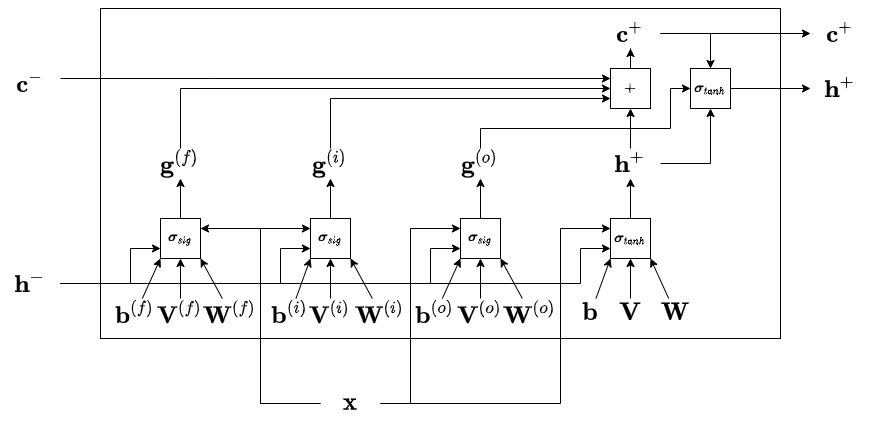
\includegraphics[width=0.8\textwidth]{"bin/LSTM.drawio.png"}
    \caption{LSTM model architecture}
    \label{fig:my_LSTM}
\end{figure}

LSTM models are highly flexible as the LSTM only refers to a single cell
that can be used in any configuration of neural network architecture.
The following hyperparameters, amongst others, can be tuned: the loss
function, the number of LSTM layers, the number of LSTM units in each
layer, the dropout rate, the number of epochs, and whether the first
LSTM layer outputs a sequence. The LSTM models were implemented using
the Keras API for Tensorflow.

\hypertarget{svr}{%
\subsection{SVR}\label{svr}}

The SVR is an extension to the Support Vector Machine for regression
problems. The SVR attempts to fit a ``hyper-tube'' in high dimensional
space around the true function which is analogous to the SVM hyperplane
(\protect\hyperlink{ref-vapnik}{Vapnik, 1999}). Observations within the
``hyper-tube'' are not penalised while observations on the
``hyper-tube'' or outside the ``hyper-tube'' are penalised and become
the support vectors for the ``hyper-tube''. By applying a basis
expansion through the use of a kernel function, the ``hyper-tube'' can
be expressed in a higher dimensional function space. This allows for
extremely non-linear ``hyper-tubes'' to be formed.

\par

The SVR can be expressed as a Lagrangian optimisation problem. The
primal optimisation problem is given as \begin{equation}\label{SVR}
    \begin{array}{ll}
    \underset{\beta_0, \boldsymbol{\tau}, \boldsymbol{\xi},\boldsymbol{\xi^* }} {\text{minimize}} & \frac{1}{2} \boldsymbol{\tau ' K \tau} + C \sum_{i=1}^N (\xi_i + \xi_i^*)\\
        \text{subject to } & \beta_0 + \sum_{j=1}^N \tau_j K(\mathbf{x}_i,\mathbf{x}_j) - y_i \leq \varepsilon + \xi_i \text{ for all } i = 1,2,...,N\\
        & y_i - \beta_0 - \sum_{j=1}^N \tau_j K(\mathbf{x}_i,\mathbf{x}_j) \leq \varepsilon + \xi_i^* \text{ for all } i = 1,2,...,N \\
        & \xi_i \geq 0 \text{ for all } i =1,2,...,N.
    \end{array}
\end{equation} The dual optimisation problem is given by

\begin{equation}
    \begin{array}{ll}
    \underset{\boldsymbol{\alpha}, \boldsymbol{\alpha^* }}{\text{maximize}} & -\varepsilon \mathbf{1}'(\boldsymbol{\alpha} + \boldsymbol{\alpha^* }) + \mathbf{y}'(\boldsymbol{\alpha^* } - \boldsymbol{\alpha})- \frac{1}{2} (\boldsymbol{\alpha^* } - \boldsymbol{\alpha})'\textbf{G}(\boldsymbol{\alpha^*} - \boldsymbol{\alpha}) \\
    & \\
    \text{subject to } & 0 \leq \alpha_i, \alpha_i^* \leq C \text{; for all } i = 1,2,...,N \\
    & \\
    \multicolumn{2}{c}{\sum_{i=1}^N (\alpha_i^* - \alpha_i) = 0}
    \end{array}
\end{equation} where
\(\mathbf{G}_{ij} = K(\mathbf{x}_i, \mathbf{x}_j).\) The optimisation of
the SVR can be achieved through quadratic programming. In the
implementation of liquidSVM, only a Gaussian radial basis function
kernel is possible. The hyperparameters for the SVR are
\(\lambda = \frac{1}{C}\) from equation \ref{SVR}. Additionally, the
hyperparameter \(\gamma\) is given as the bandwidth of the kernel.

\hypertarget{analysis}{%
\subsection{Analysis}\label{analysis}}

Since the true volatility, \(\sigma_t\), of the returns series is not
observable, a proxy was needed (\protect\hyperlink{ref-svr-GARCH}{Sun \&
Yu, 2020}). Following the framework of (\protect\hyperlink{ref-li}{Li,
Liang, Li, Wang \& Wu, 2009}), a proxy of the volatility was calculated
as the following \begin{equation}
\sigma_t = \sum_{i=0}^4 r_{t-i}
\end{equation} which is the 5-day rolling average of the squared return.
This was used as the target variable in the machine learning models. A
one-day ahead forecast and a three-day ahead forecast, where there was
an interval of two days between the inputs and the target variable, were
performed.

\par

In order to test whether a GARCH class of models was appropriate, the
autoregressive nature of the returns series, \(r_t\), squared returns
series \(r_t^2\) and the absolute value of the returns series,
\(|r_t|\), were tested using the autocorrelation functions (ACFs). Once
the autoregressive nature of the squared residuals was determined, a
AR(1) model was fit tp the return series for the mean equations. The
residuals \(\varepsilon_t\) were modelled using various GARCH models.
The AIC was used to determine which model fit best. The best fitting
model was used to forecast one-day ahead using the training and
validation sets. The performance of the forecast was determine using the
MSE given as \[
MSE = \frac{1}{N}\sum_{i=1}^N(\hat{\sigma}_t - \sigma_t)^2
\] where \(\hat{\sigma}_t\) is the forecasted volatility at time \(t\).

\par

The machine learning techniques were used for one-day ahead forecasts
and three-day ahead forecasts. For the one-day ahead forecast, the
machine learning models were trained using the
\([\sigma_{t-1}, \varepsilon_{t-1}^2]\) where \(\varepsilon_{t-1}\) is
the residual of an AR(1) process of \(r_t\)
(\protect\hyperlink{ref-svr-garch-2}{Bezerra \& Albuquerque, 2017}). For
the three day ahead forecasts, the machine learning models were trained
using the
\([\sigma_{t-1}, \sigma_{t-2}, \varepsilon_{t-1}^2, \varepsilon_{t-2}^2]\).
The performance of the forecasts of the machine learning models were
determined by MSE. The machine learning techniques were tuned for the
appropriate combination of hyperparameter using a grid-search. The
values for the grid search are given in table \ref{tab:hyp_tune}.

\begin{table}[ht]
    \centering
    \caption{Hyperparameter tuning grid}
    \begin{tabular}{lp{80mm}}
       \\[-1.8ex] \hline
\hline \\[-1.8ex] 
    Class of Models & Hyperparameters \\
    \hline \\[-1.8ex] 
        SVR & gamma: 0.082, 0.368, 1.649, 7.389, 33.115, 148.413, 665.142, 2980.958 \newline 
        lambda: 0.082, 0.368, 1.649, 7.389, 33.115, 148.413, 665.142, 2980.958 \\
        \hline \\[-1.8ex] 
        LSTM & epochs: 10, 20, 50 \newline
        loss: mse, mae \newline
                        lstm layers: 1, 2 \newline
                        lstm units: 10, 20, 40 \newline
                        return sequences: TRUE, FALSE \newline
                        dropout rate: 0, 0.1 \\
                        \hline
    \end{tabular}
    \label{tab:hyp_tune}
\end{table}

The performance of the validation forecasts were used to determine the
best hyperparameter combination. The best combinations for each class of
model were compared with the best performing model being selected for
the test set forecast. The forecast performance of the test set is given
as the overall performance.

\hypertarget{results}{%
\section{Results}\label{results}}

Following the plots in figure \ref{ret_plot}, there appears to be
periods of autoregression in the squared and absolute values of the
returns series. The ACFs are given in figure \ref{ACFs}. The
Lung-Box-Pierce Test for has a test statistic of 632.57 and a p-value of
0. The null hypothesis of no conditional heteroscedasticity in the
squared returns series was rejected. The LBQ test and GARCH-LM tests
were not conducted.

\par

An AR(1) model was used for the mean equation. Table \ref{best_mod}
shows the results of a number of different GARCH class models. Each
model was fit with GARCH(1,1) specification. The EGARCH(1,1) model had
the lowest AIC of -6.4901. The coefficients of the EGARCH(1,1) fit to
the validation set are given in table \ref{EGARCH_tab}. Plots of the
EGARCH forecasts are given in the appendix.

\par

The best hyperpameter combinations for both the one-day ahead and
three-day ahead LSTM models were: mse, 20 epochs, 2, layers, 40 units,
return sequence and dropout rate of 0. The combination of
hyperparameters had no effect on the SVR models thus the hyperparameters
were both set to 0.082.

\par

The best performing model from each class of models is given in table
\ref{tab:tune_perf}. The EGARCH(1,1) model was only used for the one-day
ahead forecasts. The LSTM model had the lowest MSE for the one-day ahead
forecasting while the SVR model had the lowest MSE for the three-day
ahead forecasting. Figure \ref{lstm_one} shows the LSTM models
performance on the validation set where the red indicates the forecasted
values and the grey is the true volatility. Figure \ref{svr_three} shows
the SVR models performance on the three-day ahead forecast. Clearly the
models were much better and predicting one-day ahead than three-days
ahead.

\begin{figure}[H]

{\centering 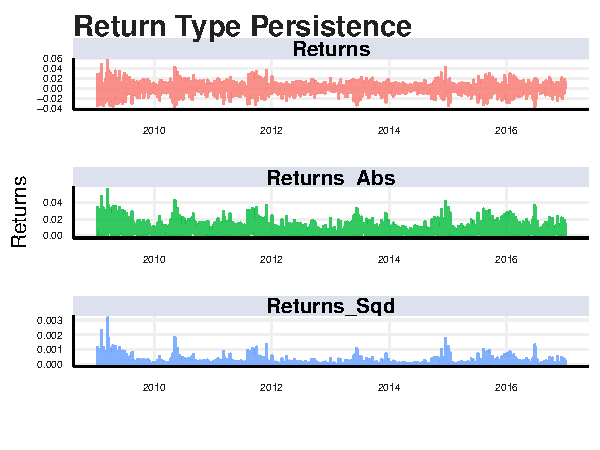
\includegraphics{Essay_files/figure-latex/garch_plot_1 -1} 

}

\caption{Plots of returns, squared returns and absolute value of returns \label{ret_plot}}\label{fig:garch_plot_1 }
\end{figure}

\begin{figure}[H]

{\centering 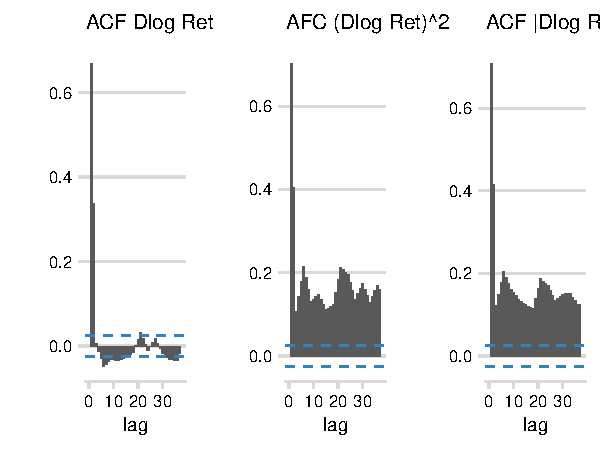
\includegraphics{Essay_files/figure-latex/garch_plot_2 -1} 

}

\caption{ACF plots of returns, squared returns and absolute value of returns \label{ACFs}}\label{fig:garch_plot_2 }
\end{figure}

\begin{table}[!htbp] \centering 
  \caption{Selection statistics of different GARCH based models} 
  \label{best_mod} 
\begin{tabular}{@{\extracolsep{5pt}} ccccc} 
\\[-1.8ex]\hline 
\hline \\[-1.8ex] 
 & sGARCH & gjrGARCH & eGARCH & apARCH \\ 
\hline \\[-1.8ex] 
Akaike & $$-$6.452$ & $$-$6.482$ & $$-$6.490$ & $$-$6.476$ \\ 
Bayes & $$-$6.439$ & $$-$6.466$ & $$-$6.474$ & $$-$6.457$ \\ 
Shibata & $$-$6.452$ & $$-$6.482$ & $$-$6.490$ & $$-$6.476$ \\ 
Hannan-Quinn & $$-$6.447$ & $$-$6.476$ & $$-$6.484$ & $$-$6.469$ \\ 
\hline \\[-1.8ex] 
\end{tabular} 
\end{table}

\begin{table}[!htbp] \centering 
  \caption{EGARCH validation model coefficients} 
  \label{EGARCH_tab} 
\begin{tabular}{@{\extracolsep{5pt}} ccccc} 
\\[-1.8ex]\hline 
\hline \\[-1.8ex] 
 &  Estimate &  Std. Error &  t value & Pr(\textgreater \textbar t\textbar ) \\ 
\hline \\[-1.8ex] 
mu & $0.0003$ & $0.0003$ & $0.951$ & $0.342$ \\ 
ar1 & $0.026$ & $0.044$ & $0.599$ & $0.549$ \\ 
omega & $$-$0.324$ & $0.007$ & $$-$46.199$ & $0$ \\ 
alpha1 & $$-$0.149$ & $0.022$ & $$-$6.639$ & $0$ \\ 
beta1 & $0.967$ & $0.0001$ & $8,874.838$ & $0$ \\ 
gamma1 & $0.061$ & $0.027$ & $2.257$ & $0.024$ \\ 
shape & $8.276$ & $2.892$ & $2.862$ & $0.004$ \\ 
\hline \\[-1.8ex] 
\end{tabular} 
\end{table}

\begin{figure}[H]

{\centering 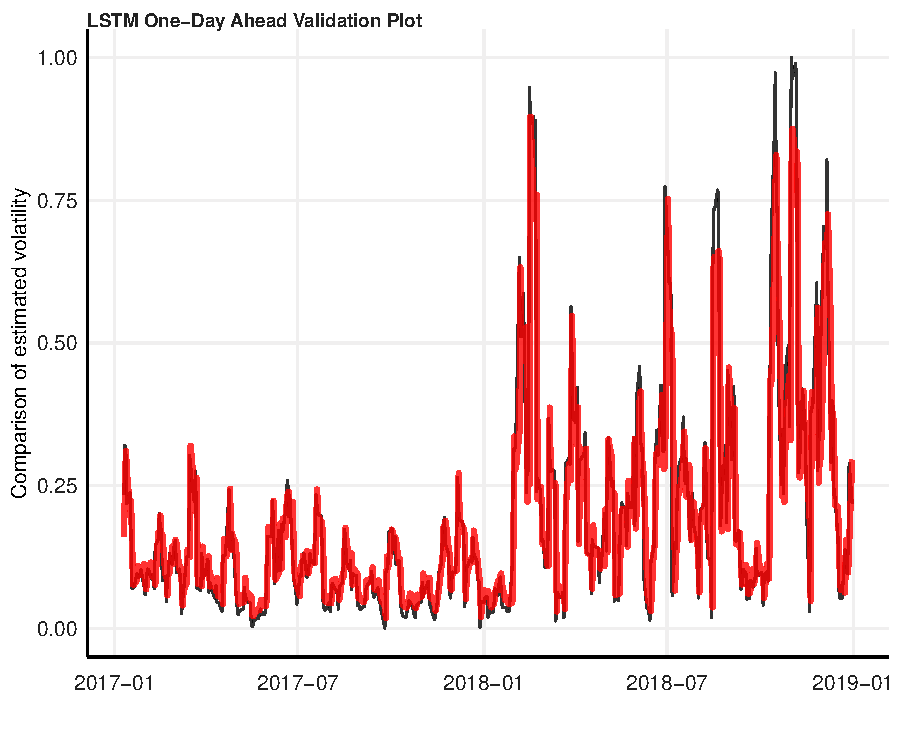
\includegraphics{Essay_files/figure-latex/plot_val-1} 

}

\caption{LSTM One-Day Ahead Validation Forecast \label{lstm_one}}\label{fig:plot_val}
\end{figure}

\begin{figure}[H]

{\centering 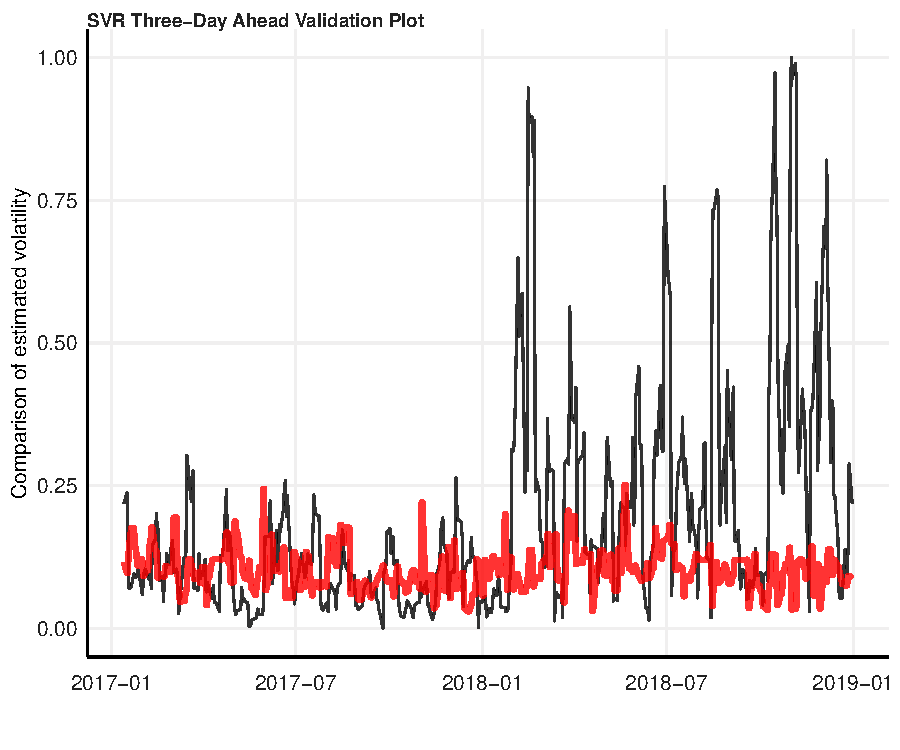
\includegraphics{Essay_files/figure-latex/plot_val_3-1} 

}

\caption{SVR Three-Day Ahead Validation Forecast \label{svr_three}}\label{fig:plot_val_3}
\end{figure}

\begin{table}[ht]
    \centering
    \caption{Best hyperparameters training and validation performance}
    \begin{tabular}{ccc}
    \\[-1.8ex]\hline 
\hline \\[-1.8ex] 
        Model & Training MSE & Validation MSE\\
        \hline \\[-1.8ex] 
        \multicolumn{3}{c}{One-day ahead} \\
        \hline
        EGARCH & 0.0115 &  0.0264 \\
        LSTM & 0.0035 & 0.0096\\
        SVR & 0.0034 & 0.0097\\
        \hline \\[-1.8ex] 
        \multicolumn{3}{c}{Three-day ahead} \\
        \hline
        LSTM & 0.0152 & 0.0477\\
        SVR & 0.0081 & 0.0462\\
        \hline \\[-1.8ex] 
    \end{tabular}
    \label{tab:tune_perf}
\end{table}

The results from the best models forecasts using the test set are given
in table \ref{tab:test_perf}. Figure \ref{lstm_test_one} shows the LSTM
model's one-day ahead test performance. Figure \ref{svr_test_three}
shows the SVR model's three-day ahead test performance. The figures
display that the one-day ahead forecast was far more precise than the
three-day ahead forecasts. This could be due to the weak autocorrelation
over that size interval. Thus the inputs three and four days prior to
the forecast date having insufficient information. Using a longer inputs
series may yield improved results especially for the LSTM which relies
on large training data sets. The poor three-day forecasting performance
illustrates the difficulty of forecasting volatility far into the
future. Recently, new artificial neural network architectures including
transformer models have offered potential to improved volatility
forecasting results
(\protect\hyperlink{ref-vol-transformer}{Ramos-Pérez, Alonso-González \&
Núñez-Velázquez, 2021}).

\begin{figure}[H]

{\centering 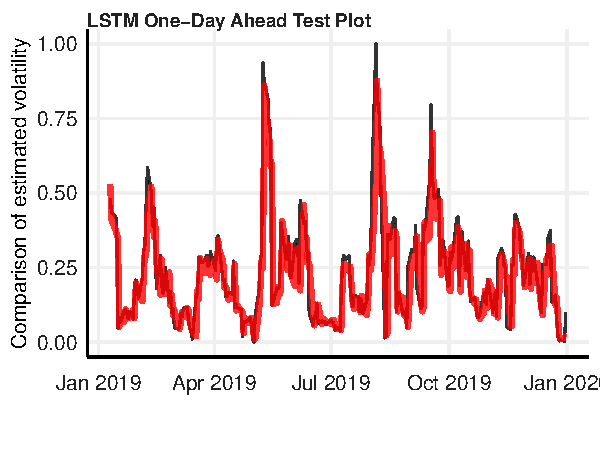
\includegraphics{Essay_files/figure-latex/plot_test-1} 

}

\caption{LSTM One-Day Ahead Test Forecast \label{lstm_test_one}}\label{fig:plot_test}
\end{figure}

\begin{table}[ht]
    \centering
    \caption{Forecasting full training and test performance}
    \begin{tabular}{ccc}
    \\[-1.8ex]\hline 
\hline \\[-1.8ex] 
        Model & Full Training MSE & Test MSE\\
        \hline
        \multicolumn{3}{c}{One-day ahead} \\
        \hline
        LSTM & 0.0031 & 0.0121\\
        \hline \\[-1.8ex] 
        \multicolumn{3}{c}{Three-day ahead} \\
        \hline
        SVR & 0.0037 & 0.0523\\
        \hline \\[-1.8ex] 
    \end{tabular}
    \label{tab:test_perf}
\end{table}

\begin{figure}[H]

{\centering 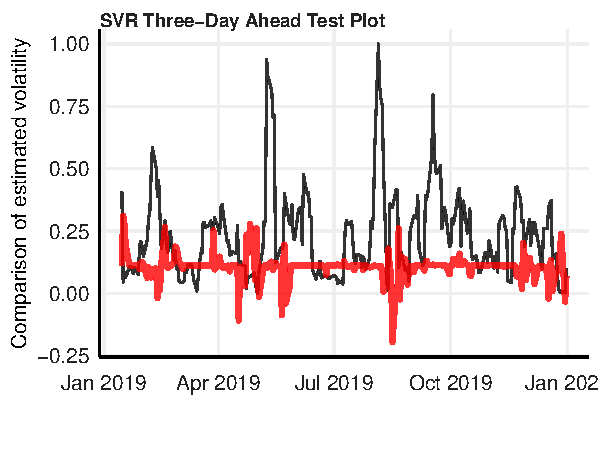
\includegraphics{Essay_files/figure-latex/plot_3_test-1} 

}

\caption{LSTM Three-Day Ahead Test Forecast \label{svr_test_three}}\label{fig:plot_3_test}
\end{figure}

\hypertarget{conclusion}{%
\section{Conclusion}\label{conclusion}}

While forecasting returns series is of little use due to the potential
for arbitrage opportunities, forecasting volatility is an important task
in financial econometrics. In this paper, three different classes of
volatility models were compared. For one-day ahead volatility modelling,
the LSTM model performs best with the lowest MSE. The plots of the
forecasts illustrate a very close fit to the data. For three-day ahead
forecasting, the SVR model performs best. However, as illustrated by
plots of the forecasts, the three-day ahead forecasts do not perform as
well. The novel approach to using these machine learning techniques to
the South African context show that their high levels of performance
translates to this context. While volatility modelling, especially with
long time intervals, still posses a significant challenge, machine
learning techniques offer a method for more accurate forecasting.

\newpage

\hypertarget{references}{%
\section*{References}\label{references}}
\addcontentsline{toc}{section}{References}

\hypertarget{refs}{}
\begin{CSLReferences}{1}{0}
\leavevmode\hypertarget{ref-sa_garch}{}%
Babikir, A., Gupta, R., Mwabutwa, C. \& Owusu-Sekyere, E. 2012.
Structural breaks and GARCH models of stock return volatility: The case
of south africa. \emph{Economic Modelling}. 29(6):2435--2443.

\leavevmode\hypertarget{ref-svr-garch-2}{}%
Bezerra, P.C.S. \& Albuquerque, P.H.M. 2017. Volatility forecasting via
SVR--GARCH with mixture of gaussian kernels. \emph{Computational
Management Science}. 14(2):179--196.

\leavevmode\hypertarget{ref-sa-gold}{}%
Chai, J., Zhao, C., Hu, Y. \& Zhang, Z.G. 2021. Structural analysis and
forecast of gold price returns. \emph{Journal of Management Science and
Engineering}. 6(2):135--145.

\leavevmode\hypertarget{ref-engle}{}%
Engle, R.F. 1982. Autoregressive conditional heteroscedasticity with
estimates of the variance of united kingdom inflation.
\emph{Econometrica: Journal of the econometric society}. 987--1007.

\leavevmode\hypertarget{ref-lstm}{}%
Gers, F.A., Schmidhuber, J. \& Cummins, F. 2000. Learning to forget:
Continual prediction with LSTM. \emph{Neural computation}.
12(10):2451--2471.

\leavevmode\hypertarget{ref-lit_ml}{}%
Henrique, B.M., Sobreiro, V.A. \& Kimura, H. 2019. Literature review:
Machine learning techniques applied to financial market prediction.
\emph{Expert Systems with Applications}. 124:226--251.

\leavevmode\hypertarget{ref-sa-garch2}{}%
Ismail, M.T., Audu, B. \& Tumala, M.M. 2016. Volatility forecasting with
the wavelet transformation algorithm garch model: Evidence from african
stock markets. \emph{The Journal of Finance and Data Science}.
2(2):125--135.

\leavevmode\hypertarget{ref-li}{}%
Li, N., Liang, X., Li, X., Wang, C. \& Wu, D.D. 2009. Network
environment and financial risk using machine learning and sentiment
analysis. \emph{Human and Ecological Risk Assessment}. 15(2):227--252.

\leavevmode\hypertarget{ref-LIU}{}%
Liu, Y. 2019. Novel volatility forecasting using deep learning--long
short term memory recurrent neural networks. \emph{Expert Systems with
Applications}. 132:99--109.

\leavevmode\hypertarget{ref-nelson}{}%
Nelson, D.B. 1991. Conditional heteroskedasticity in asset returns: A
new approach. \emph{Econometrica}. 59(2):347--370. {[}Online{]},
Available: \url{http://www.jstor.org/stable/2938260}.

\leavevmode\hypertarget{ref-svr_garch}{}%
Pérez-Cruz, F., Afonso-Rodriguez, J.A. \& Giner, J. 2003. Estimating
GARCH models using support vector machines. \emph{Quantitative Finance}.
3(3):163.

\leavevmode\hypertarget{ref-vol-transformer}{}%
Ramos-Pérez, E., Alonso-González, P.J. \& Núñez-Velázquez, J.J. 2021.
Multi-transformer: A new neural network-based architecture for
forecasting s\&p volatility. \emph{Mathematics}. 9(15):1794.

\leavevmode\hypertarget{ref-ann}{}%
Sheta, A.F., Ahmed, S.E.M. \& Faris, H. 2015. A comparison between
regression, artificial neural networks and support vector machines for
predicting stock market index. \emph{Soft Computing}. 7(8):2.

\leavevmode\hypertarget{ref-svr-GARCH}{}%
Sun, H. \& Yu, B. 2020. Forecasting financial returns volatility: A
GARCH-SVR model. \emph{Computational Economics}. 55(2):451--471.

\leavevmode\hypertarget{ref-tsay}{}%
Tsay, R. 2012.

\leavevmode\hypertarget{ref-vapnik}{}%
Vapnik, V. 1999. \emph{The nature of statistical learning theory}.
Springer science \& business media.

\end{CSLReferences}

\hypertarget{appendix}{%
\section*{Appendix}\label{appendix}}
\addcontentsline{toc}{section}{Appendix}

\begin{figure}[H]

{\centering 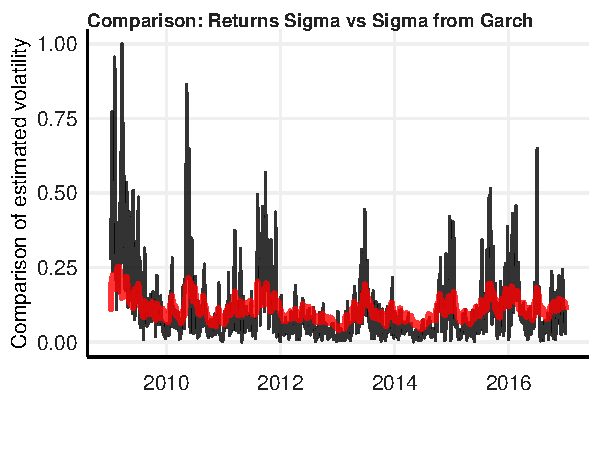
\includegraphics{Essay_files/figure-latex/plot_1-1} 

}

\caption{EGARCH(1,1) One-Day Ahead Training Forecast}\label{fig:plot_1}
\end{figure}

\begin{figure}[H]

{\centering 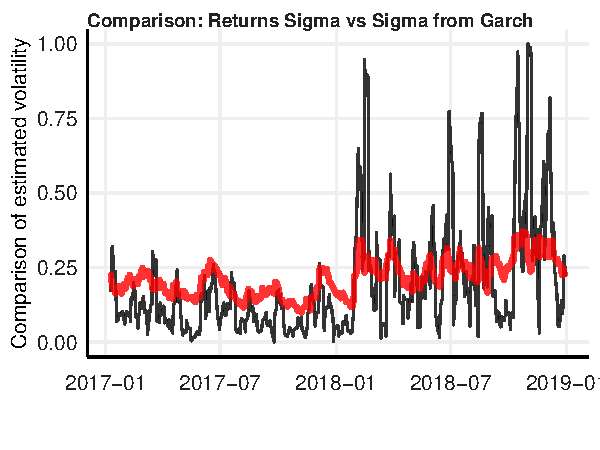
\includegraphics{Essay_files/figure-latex/plot_2-1} 

}

\caption{EGARCH(1,1) One-Day Ahead Validation Forecast}\label{fig:plot_2}
\end{figure}

\begin{figure}[H]

{\centering 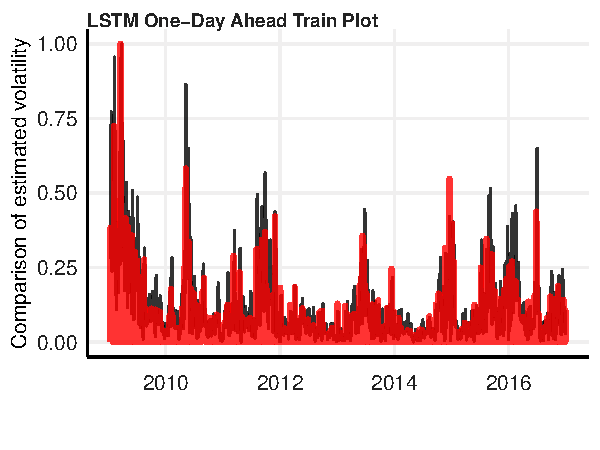
\includegraphics{Essay_files/figure-latex/plot_3-1} 

}

\caption{LSTM One-Day Ahead Training Forecast}\label{fig:plot_3}
\end{figure}

\begin{figure}[H]

{\centering 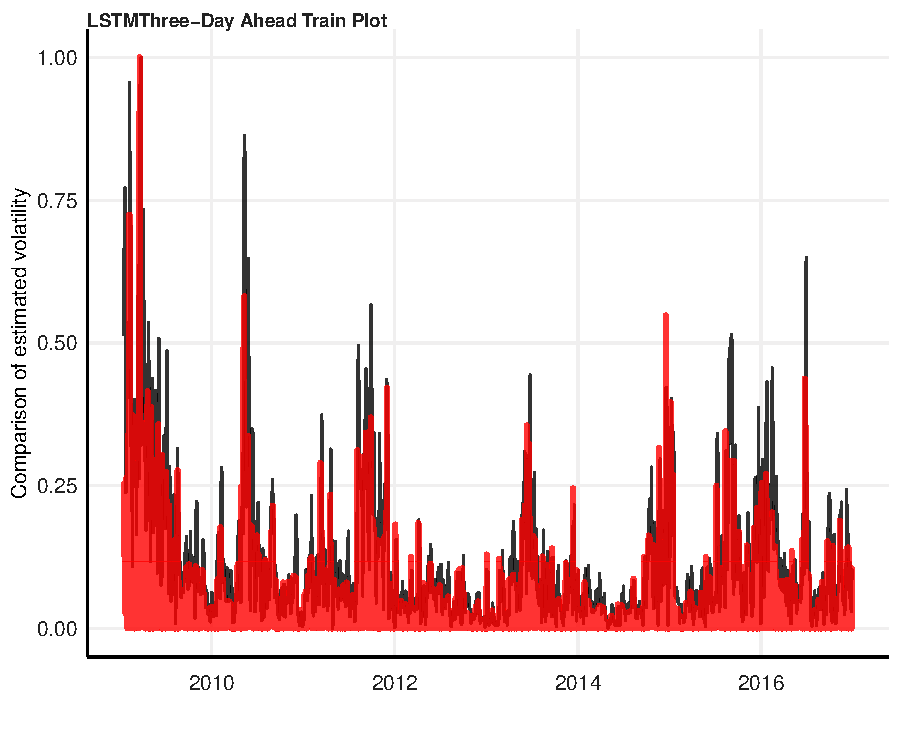
\includegraphics{Essay_files/figure-latex/plot_4-1} 

}

\caption{LSTM Three-Day Ahead Training Forecast}\label{fig:plot_4}
\end{figure}

\begin{figure}[H]

{\centering 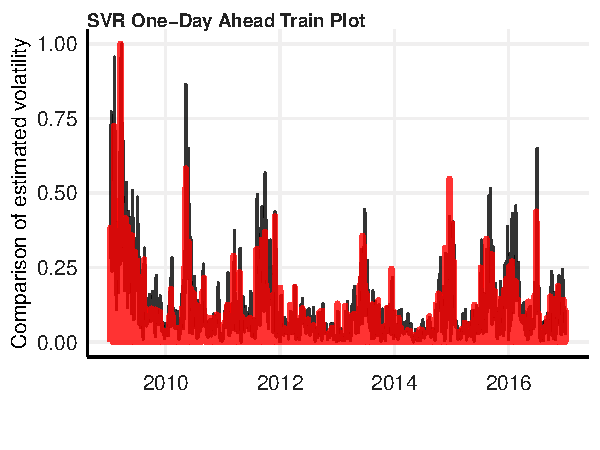
\includegraphics{Essay_files/figure-latex/plot_5-1} 

}

\caption{SVR One-Day Ahead Training Forecast}\label{fig:plot_5}
\end{figure}

\begin{figure}[H]

{\centering 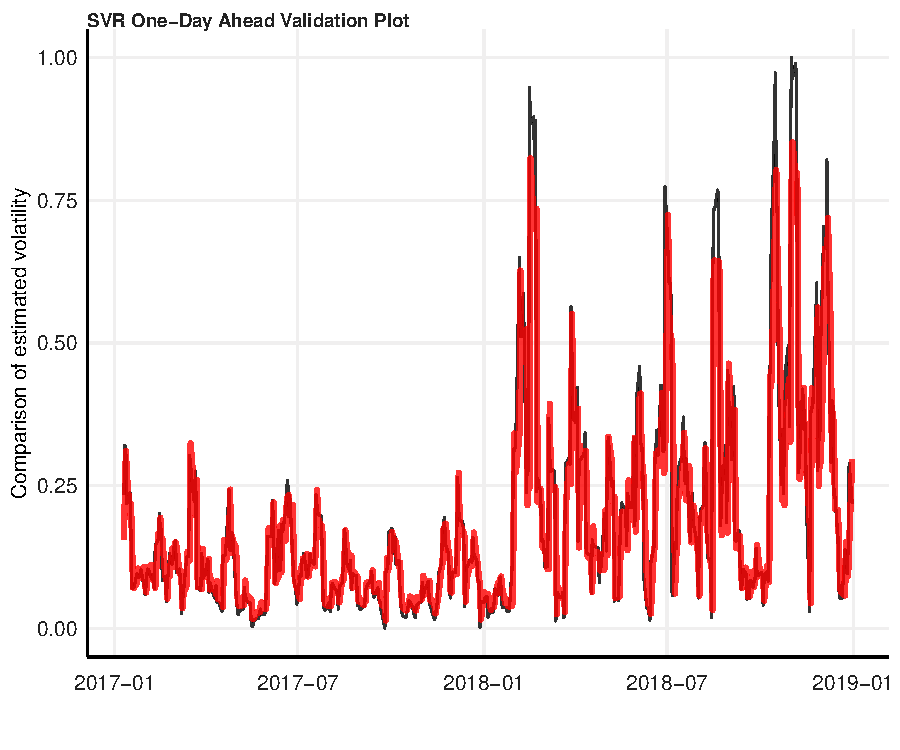
\includegraphics{Essay_files/figure-latex/plot_6-1} 

}

\caption{SVR One-Day Ahead Validation Forecast}\label{fig:plot_6}
\end{figure}

\begin{figure}[H]

{\centering 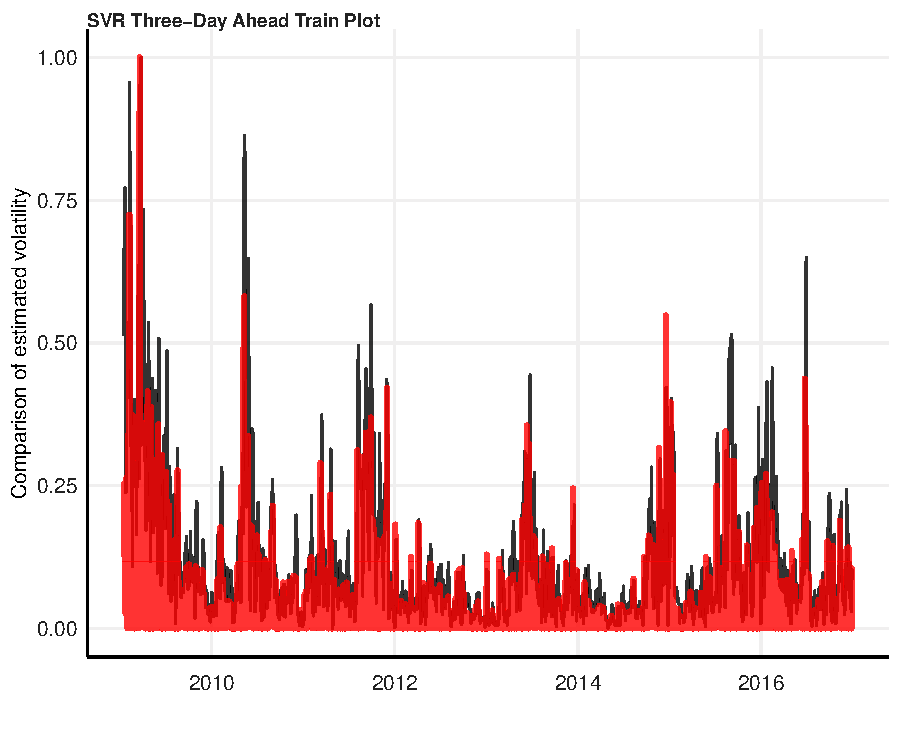
\includegraphics{Essay_files/figure-latex/plot_7-1} 

}

\caption{SVR Three-Day Ahead Training Forecast}\label{fig:plot_7}
\end{figure}

\begin{figure}[H]

{\centering 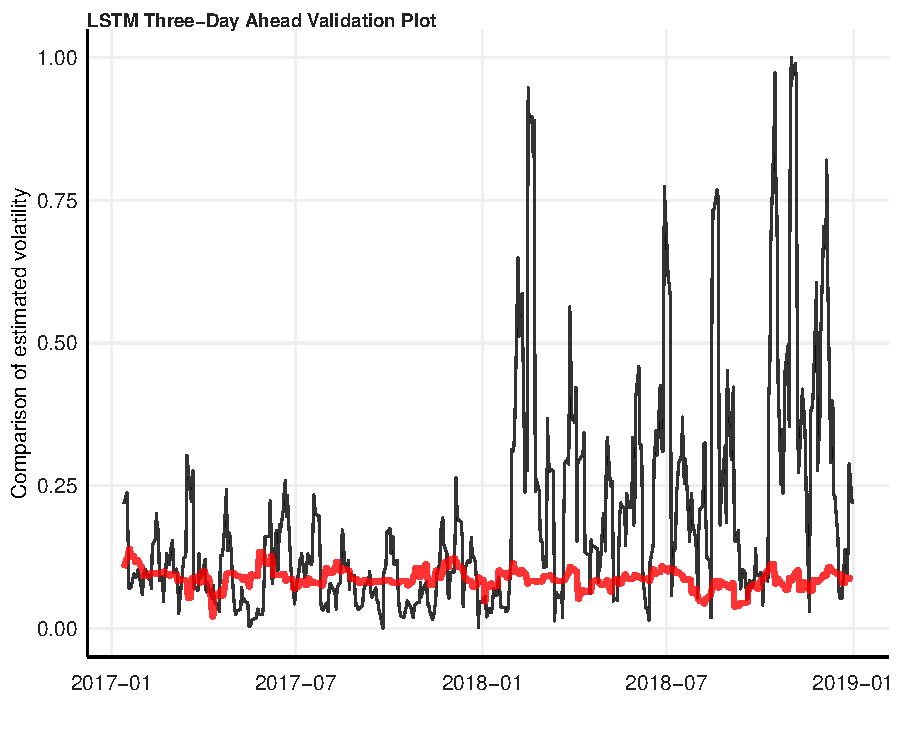
\includegraphics{Essay_files/figure-latex/plot_8-1} 

}

\caption{LSTM Three-Day Ahead Validation Forecast}\label{fig:plot_8}
\end{figure}

\begin{figure}[H]

{\centering 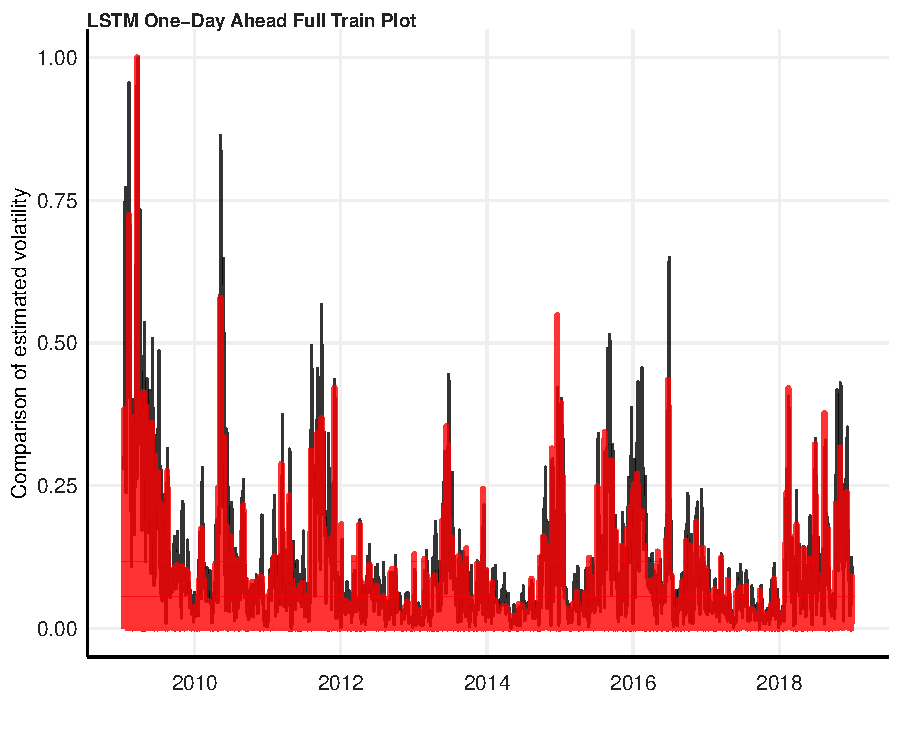
\includegraphics{Essay_files/figure-latex/plot_9-1} 

}

\caption{LSTM One-Day Ahead Full Training Forecast}\label{fig:plot_9}
\end{figure}

\begin{figure}[H]

{\centering 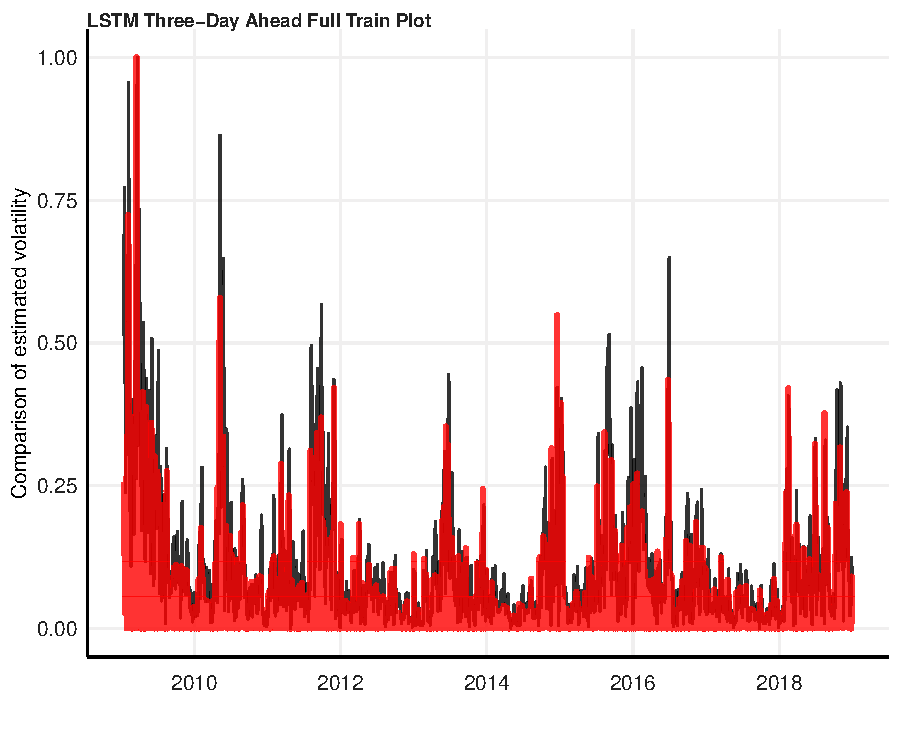
\includegraphics{Essay_files/figure-latex/plot_10-1} 

}

\caption{SVR Three-Day Ahead Full Training Forecast}\label{fig:plot_10}
\end{figure}

\bibliography{Tex/ref}





\end{document}
